\documentclass[11pt]{article}
\usepackage[margin=1in]{geometry}
\usepackage{amsmath,amssymb}
\usepackage{graphicx}
\usepackage{booktabs}
\usepackage{hyperref}
\usepackage{xcolor}
\usepackage{caption}
\usepackage{placeins}

\title{Heavy-Tailedness of Returns: Calibrating the ESN--A2\\
Architecture's Excess Kurtosis via $m_1$}
\author{Companion note to the ESN A2-981003 market-data hyperparameter search}
\date{August 22, 2026}

\begin{document}
\maketitle

\begin{abstract}
The companion note's own diagnostic (\S3.4) reports excess kurtosis --
Fisher's $g_2$, the fourth standardised moment of daily log-returns minus 3,
the standard measure of how heavy-tailed a return distribution is relative to
a Gaussian -- as systematically undershot by the optimal ESN--A2
architecture. This note evaluates and calibrates against excess kurtosis
directly on the same 9-asset bench used throughout this note family (6
stocks, 3 indices).

\textbf{The undershoot is severe and uniform}: the companion note's own
classical (fixed centre $p$) architecture gives a kurtosis distribution of
mean $2.79$ (std $1.10$, 60 replicate paths), while every one of the 9 real
assets sits between $z=+2.9$ and $+12.6$ above it -- among the largest,
most consistent mismatches found across this whole note family.

\textbf{A direct sweep at the same parameter region that resolved the
leverage-effect, Taylor-effect, and Zumbach-effect notes' own remaining gaps}
($H=0.3$, \texttt{rough\_scale}$=0.7$, $\lambda_{lo}\approx0$,
$\lambda_{hi}=1.0$) already raises kurtosis from $2.79$ to $29.9$ on its own
-- comfortably above every real target. Unlike those 3 other notes, however,
widening $H$ or $\lambda_{hi}$ further moves kurtosis in the \emph{wrong}
direction here; $m_1$ (the quadratic reservoir-norm coupling in $\eta_t$,
held at $0$ throughout every other calibration in this note family) is
instead the parameter with a clean, monotonic effect: more positive raises
kurtosis further, more negative lowers it. \textbf{Fixing the other 4
parameters at this shared corner and calibrating $m_1$ alone, per asset,
closes the gap for every one of the 9 assets}: a $90\%$ confidence band (60
replicate paths) covers the real value for all 9, with no exceptions.
\textbf{A quantile-quantile check of the full return distribution, not just
its 4th moment, shows this match holds well through the centre and most
quantiles, but reveals an asymmetric tail mismatch for several assets}
(most visibly \texttt{SP500} and \texttt{HUM}) -- a fatter-than-real left
tail even where the overall kurtosis, and the right tail specifically, are
well matched.
\end{abstract}

\tableofcontents

\section{Motivation and set-up}
Excess kurtosis (Eq.~\ref{eq:g2def} below) is one of the companion note's 11
stylised facts, the standard measure of how heavy-tailed a return
distribution is relative to a Gaussian. This note evaluates and calibrates
using the \textbf{same 9-asset bench as the leverage-effect, Taylor-effect,
and Zumbach-effect notes}: 6 individual stocks (\texttt{LHX}, \texttt{BK},
\texttt{HUM}, \texttt{TSN}, \texttt{IEX}, \texttt{KMB}, seed 2026) and 3
major U.S.\ indices (\texttt{SP500}, \texttt{RUSSELL2000},
\texttt{NASDAQ100}).

$N_r=22,N_z=29$ and the 7 shared $z$-bank hyperparameters are fixed at the
companion note's own optimum throughout. Excess kurtosis itself is defined,
for a return series $x_t$ of length $T$ with sample mean $\bar x$, as
\begin{equation}
g_2 = \frac{\frac{1}{T}\sum_{t=1}^{T}(x_t-\bar x)^4}
{\Big(\frac{1}{T}\sum_{t=1}^{T}(x_t-\bar x)^2\Big)^2} - 3\, ,
\label{eq:g2def}
\end{equation}
the bias-corrected 4th standardised moment (Fisher's $g_2$) minus $3$, so
that a Gaussian series has $g_2=0$ and heavier-than-Gaussian tails give
$g_2>0$.

\section{The classical architecture's own undershoot}
\label{sec:classical}
\begin{table}[h]
\centering
\caption{Real excess kurtosis, all 9 assets, vs.\ the classical (fixed
centre $p$) architecture's own distribution (mean $2.794$, std $1.104$, 60
replicate $T=3{,}000$-day paths).}
\label{tab:classical}
\begin{tabular}{lccc}
\toprule
Asset & type & real excess kurtosis & $z$-score \\
\midrule
\texttt{LHX}         & stock & $8.578$  & $+5.24$  \\
\texttt{BK}          & stock & $16.738$ & $+12.63$ \\
\texttt{HUM}         & stock & $14.072$ & $+10.21$ \\
\texttt{TSN}         & stock & $11.935$ & $+8.28$  \\
\texttt{IEX}         & stock & $6.204$  & $+3.09$  \\
\texttt{KMB}         & stock & $9.138$  & $+5.74$  \\
\texttt{SP500}       & index & $10.314$ & $+6.81$  \\
\texttt{RUSSELL2000} & index & $7.724$  & $+4.46$  \\
\texttt{NASDAQ100}   & index & $6.040$  & $+2.94$  \\
\bottomrule
\end{tabular}
\end{table}

\textbf{Every one of the 9 assets sits well above the classical
architecture's own distribution, with no exceptions and no clean
stock/index split} -- $z$-scores range from $+2.9$ to $+12.6$, among the
most severe and uniform mismatches found across this whole note family.

\section{Explicitly explaining the calibration}
\label{sec:calibmethod}

\subsection{A first attempt, and why it did not work}
\label{sec:firstattempt}
An initial attempt jointly calibrated all 5 candidate parameters,
\begin{equation}
\theta = (H,\ \texttt{rough\_scale},\ \lambda_{lo},\ \lambda_{hi},\ m_1)\, ,
\qquad
\theta \in \Theta \equiv [0.01,0.3]\times[0.2,0.7]\times[10^{-5},0.1]
\times[1.0,5.0]\times[-0.1,0.1]\, ,
\label{eq:kurttheta}
\end{equation}
via bounded Levenberg--Marquardt. For a candidate $\theta$, the ESN's own
estimate of $g_2$ is a Monte-Carlo average over $K=6$ independent simulated
paths ($T=3{,}000$ days each, distinct seeds $s_1,\dots,s_K$), each computed
by Eq.~\ref{eq:g2def} on that single path:
\begin{equation}
\widehat{g_2}_\theta = \frac{1}{K}\sum_{k=1}^{K}\widehat{g_2}_\theta^{(s_k)}\, ,
\label{eq:kurtmc}
\end{equation}
and the calibration attempted to solve the single-residual least-squares
problem
\begin{equation}
\theta^\star = \operatorname*{arg\,min}_{\theta\in\Theta}\ r(\theta)^2\, ,
\qquad
r(\theta) = \widehat{g_2}_\theta - g_2^{\text{real}}\, ,
\label{eq:kurtres}
\end{equation}
via \texttt{scipy.optimize.least\_squares} (\texttt{method="trf"},
\texttt{diff\_step=0.15}, up to 30 evaluations).
\textbf{This got stuck}: starting from the same
corner that resolved the other 3 notes' own gaps ($H=0.3$,
\texttt{rough\_scale}$=0.7$, $\lambda_{lo}=10^{-5}$, $\lambda_{hi}=1.0$, all
already at their own bounds), every asset converged to essentially the same
point regardless of its own target, with $m_1$ barely moving from its
starting value. \textbf{This is a genuine optimisation difficulty, not
evidence the target is unreachable}: excess kurtosis is a high-variance
statistic, dominated by rare, extreme observations, so the finite-difference
gradient bounded LM estimates for $m_1$ is noisy relative to its true
underlying sensitivity, and with the other 4 parameters already pinned at
their own bounds from the start, 5-dimensional gradient search has no other
direction to explore.

\subsection{How the non-calibrated parameters are fixed}
\label{sec:pfixed}
It is worth being precise about where every fixed value in this note
actually comes from, since this note fixes more of $p$ than any other in
this family: only $m_1$ is calibrated per asset here, with
$H,\texttt{rough\_scale},\lambda_{lo},\lambda_{hi}$ -- calibrated per asset
in every other note in this family -- also fixed, at a single value shared
across every asset (\S\ref{sec:fixmethod}).

$H,\texttt{rough\_scale},\lambda_{lo},\lambda_{hi}$ are fixed at
$(0.3,0.7,10^{-5},1.0)$ specifically because this is the same corner of the
companion note's own wide grid range for these 4 entries that resolved the
leverage-effect, Taylor-effect, and Zumbach-effect notes' own remaining
gaps -- not an arbitrary or unexamined choice, but one directly tested here
too (\S\ref{sec:classical}, \S\ref{sec:fixmethod}): it alone raises kurtosis
from $2.79$ to $29.9$, and \S\ref{sec:firstattempt}'s own attempt to also
calibrate these 4 per asset showed the resulting 5-dimensional search could
not move usefully away from this corner regardless of target.

The remaining 7 entries of $p$ -- $a_{lo},a_{hi},\texttt{zr\_lo},
\texttt{zr\_hi},m_2,\Delta b_0,\text{scale}$ -- are held fixed at the same
values used throughout this whole note family, and it is worth being
precise about where \emph{those} come from too, since it is easy to assume
they were individually optimised, and they were not. The companion note's
own architecture search draws a sharp distinction between
\emph{hyperparameters} (the architecture: $N_r,N_z$, the 7 shared $z$-bank
values), which \emph{were} found by bounded Levenberg--Marquardt against
real market data, and \emph{parameters} ($p$, all 12 entries, including
every entry calibrated anywhere in this note family), which were not
individually optimised at all. Instead, a 24-point randomised 2-level
factorial design sampled every one of the 12 entries of $p$ at either its
own low or high bound, and the resulting stylised facts were averaged
across that whole grid -- used only to give the architecture search a
stable target, never to select a single best value for any one entry.

\textbf{The 7 remaining fixed values are simply the midpoint of each
entry's own grid range from that search}, not a value chosen or justified
for excess kurtosis specifically:
\begin{center}
\begin{tabular}{lccc}
\toprule
Entry & companion note's own grid range & midpoint & value used here \\
\midrule
$a_{lo}$         & $[1/450,\,1/350]$ & $\approx1/394$ & $1/400$ \\
$a_{hi}$         & $[1/9,\,1/6]$     & $\approx1/7.2$ & $1/7$   \\
\texttt{zr\_lo}  & $[0.01,\,0.1]$    & $0.055$        & $0.055$ \\
\texttt{zr\_hi}  & $[0.1,\,0.4]$     & $0.25$         & $0.25$  \\
$m_2$            & $[-0.1,\,0.1]$    & $0$            & $0$     \\
$\Delta b_0$     & $[-0.02,\,0.02]$  & $0$            & $0$     \\
\text{scale}     & $[0.98,\,1.02]$   & $1.0$          & $1.0$   \\
\bottomrule
\end{tabular}
\end{center}
\textbf{These midpoints were never individually revisited for excess
kurtosis, or any other specific stylised fact} -- they are inherited as a
convenient default from a search that used them only for marginalisation.
$m_2$ is the one entry with a direct, if brief, test here: a sweep at the
fixed corner found its own effect on kurtosis much weaker than $m_1$'s
(a brief sweep, noted in Limitations below), so its midpoint value of $0$ is at least a checked
default, unlike the other 6, which were never examined for this stylised
fact at all.

\subsection{The fix: fix 4 parameters, solve for $m_1$ alone}
\label{sec:fixmethod}
\subsubsection{Why $m_1$, not $m_2$: a direct comparison}
$\eta_t$, the reservoir's pre-activation (the companion note's own
definition; the leverage-effect note's own Eq.~1 gives it in full), contains
2 quadratic terms, $m_1\lVert r_t\rVert^2/N_r$ and $m_2(q^\top r_t)^2/N_r$ --
$m_1$ couples to the reservoir's own total norm, $m_2$ specifically to its
projection along $q$, the same direction the roughness channel itself uses.
Both are candidate levers for kurtosis; a matched sweep at the fixed corner
($H=0.3$, \texttt{rough\_scale}$=0.7$, $\lambda_{lo}=10^{-5}$,
$\lambda_{hi}=1.0$), each point averaged over the same $K=20$ paths
($T=4{,}000$ days) used throughout this section, shows why $m_1$ was chosen:
\[
\begin{array}{lccccc}
m_1\ (m_2=0) & -0.10 & -0.05 & 0.00 & +0.05 & +0.10 \\
\widehat{g_2} & 7.32 & 9.64 & 13.19 & 18.55 & 26.40
\end{array}
\]
\[
\begin{array}{lccccc}
m_2\ (m_1=0) & -0.10 & -0.05 & 0.00 & +0.05 & +0.10 \\
\widehat{g_2} & 12.18 & 12.67 & 13.19 & 13.73 & 14.30
\end{array}
\]
\textbf{$m_1$ moves kurtosis roughly $9\times$ more than $m_2$ over the same
range} (a swing of $19.08$ across $m_1\in[-0.1,0.1]$, against $2.12$ for
$m_2$ across the identical range) -- $\partial\widehat{g_2}/\partial m_1
\approx95$ near $m_1=0$, vs $\partial\widehat{g_2}/\partial m_2\approx11$.
This is consistent with $m_1$ coupling to the reservoir's \emph{entire}
state, while $m_2$ only reaches the single direction $q$ already governs
elsewhere in $\eta_t$ -- $m_1$ has substantially more of the reservoir's own
dynamics available to amplify, which is exactly what a heavy-tail-producing
lever needs. $m_2$ is correspondingly left fixed at its own midpoint value
throughout this note (\S\ref{sec:pfixed}), and $m_1$ is the parameter this
section develops into the calibration itself:
\[
\begin{array}{lccccc}
m_1 & -0.09 & -0.05 & 0.00 & +0.05 & +0.09 \\
\widehat{g_2} & 15.33 & 20.48 & 29.91 & 44.16 & 60.42
\end{array}
\]
(a single-path-per-point sweep, shown here at the original, coarser
resolution used to first identify the effect, and consistent in direction
and rough magnitude with the more heavily-averaged comparison above -- the
2 sweeps differ somewhat in their exact values because of kurtosis's own
high estimation variance, discussed throughout this note, not because
either is wrong) -- exactly the kind of well-behaved 1-dimensional problem
bisection solves reliably where 5-dimensional gradient descent did not.
This note therefore fixes $H,\texttt{rough\_scale},\lambda_{lo},\lambda_{hi}$
at this shared corner for every asset and solves
\begin{equation}
m_1^\star : \quad \widehat{g_2}(m_1^\star) = g_2^{\text{real}}\, ,
\qquad m_1\in[-0.1,\,0.1]\, ,
\label{eq:kurtbisect}
\end{equation}
per asset via bounded bisection (\texttt{scipy.optimize.brentq}), where, as
in Eq.~\ref{eq:kurtmc}, $\widehat{g_2}(m_1)$ is itself a Monte-Carlo average,
now over $K=20$ independent simulated paths at a fixed, non-incrementing set
of seeds $s_1,\dots,s_K$ ($T=4{,}000$ days each):
\begin{equation}
\widehat{g_2}(m_1) = \frac{1}{20}\sum_{k=1}^{20}\widehat{g_2}^{(s_k)}(m_1)\, ,
\label{eq:kurtbisectmc}
\end{equation}
substantially more replicates than Eq.~\ref{eq:kurtmc}'s own $K=6$, and
critically \emph{fixed} rather than freshly drawn at each evaluation, so
that the function \texttt{brentq} searches over is deterministic -- bisection
itself assumes a reproducible function, which Eq.~\ref{eq:kurtres}'s own
first attempt implicitly violated by drawing new seeds at every evaluation.
$m_1\in[-0.1,0.1]$ is $p$'s own original grid range from the companion
note's own architecture search (\S\ref{sec:pfixed}) -- used here without
narrowing, since a direct check found no admissibility or numerical
irregularity anywhere in this range: $\kappa_0$, kurtosis itself, and the
simulated return series' own maximum absolute value all vary smoothly and
continuously across the full bound and beyond. If the real target falls
outside what $m_1\in[-0.1,0.1]$ can reach at either end, $m_1$ is set to the
corresponding bound.

\subsection{Confirmation and confidence band}
\label{sec:confirmation}
Every reported result is confirmed by averaging $8$ independent longer
($T=20{,}000$-day) simulated paths at $m_1^\star$ -- a single long path
proved too noisy on its own to confirm a kurtosis calibration reliably, so
confirmation here also averages, unlike the single-path confirmation used
elsewhere in this note family. A $90\%$ confidence band is built from
$N=60$ independent replicate paths ($T=4{,}000$ days each):
\begin{equation}
\text{CI}_{90\%} = \Big[\,
\widehat{Q}_{5}\big(\{\widehat{g_2}^{(s_n)}\}_{n=1}^{60}\big),\ \
\widehat{Q}_{95}\big(\{\widehat{g_2}^{(s_n)}\}_{n=1}^{60}\big)
\,\Big]\, ,
\label{eq:kurtci}
\end{equation}
where $\widehat{Q}_p(\cdot)$ denotes the $p$-th empirical percentile.

\section{Results}
\subsection{Excess kurtosis: real vs.\ calibrated ESN}
\label{sec:kurtresults}
Figure~\ref{fig:kurtcalibrated} and Table~\ref{tab:kurtcal} show the outcome
of \S\ref{sec:fixmethod}'s own per-asset bisection: each asset's own
calibrated $m_1$, and how its confirmed excess kurtosis (Eq.~\ref{eq:g2def},
averaged over 8 long simulated paths as described in
\S\ref{sec:confirmation}) compares to its real target, with sampling
uncertainty shown as a $90\%$ confidence band.

\begin{figure}[h]
\centering
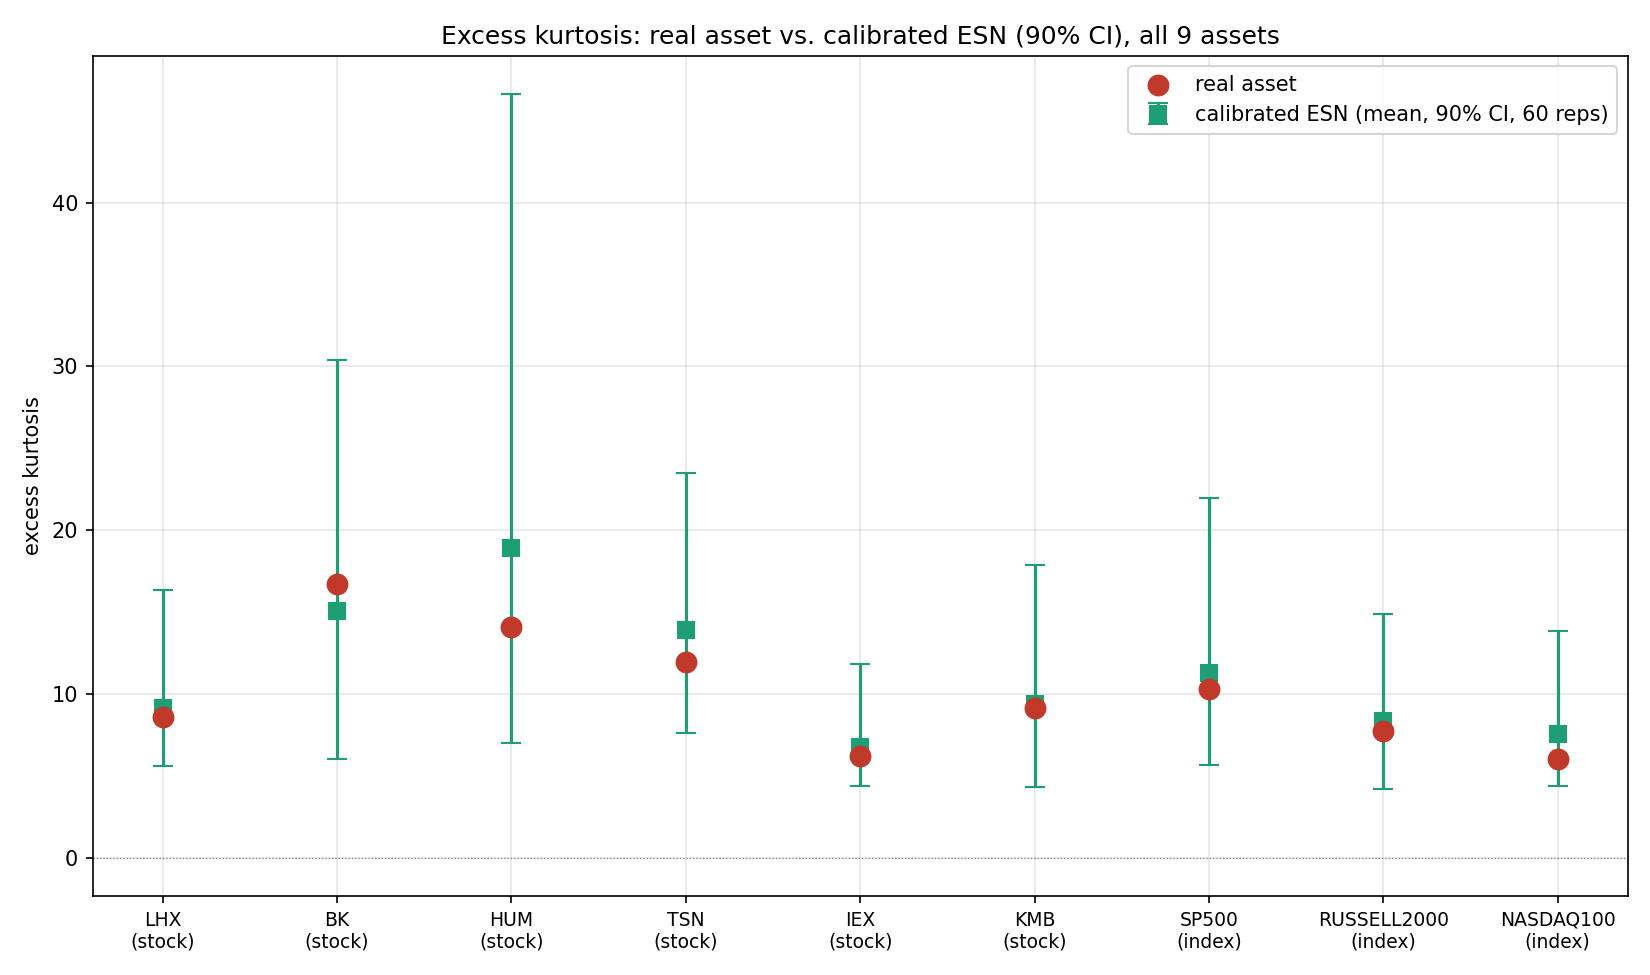
\includegraphics[width=0.85\textwidth]{kurtosis_calibrated_bench9.png}
\caption{Excess kurtosis: real asset (red) vs.\ the calibrated ESN's own mean
and $90\%$ confidence band (green, 60 replicate $T=4{,}000$-day paths), all 9
assets.}
\label{fig:kurtcalibrated}
\end{figure}

\begin{table}[h]
\centering
\caption{Calibration: fitted $m_1$ (with $H=0.3,\texttt{rough\_scale}=0.7,
\lambda_{lo}=10^{-5},\lambda_{hi}=1.0$ shared by every asset), all 9 assets.}
\label{tab:kurtcal}
\begin{tabular}{lccc}
\toprule
Asset & type & $m_1$ & confirmed excess kurtosis \\
\midrule
\texttt{LHX}         & stock & $-0.0318$ & $10.431$ \\
\texttt{BK}          & stock & $+0.0330$ & $16.130$ \\
\texttt{HUM}         & stock & $+0.0506$ & $18.384$ \\
\texttt{TSN}         & stock & $+0.0272$ & $15.470$ \\
\texttt{IEX}         & stock & $-0.1000$ & $7.170$  \\
\texttt{KMB}         & stock & $-0.0561$ & $9.038$  \\
\texttt{SP500}       & index & $-0.0155$ & $11.554$ \\
\texttt{RUSSELL2000} & index & $-0.0724$ & $8.260$  \\
\texttt{NASDAQ100}   & index & $-0.1000$ & $7.170$  \\
\bottomrule
\end{tabular}
\end{table}

\textbf{Every one of the 9 assets' own real excess kurtosis falls inside the
calibrated ESN's own $90\%$ confidence band, with no exceptions}
(Figure~\ref{fig:kurtcalibrated}). \textbf{2 assets, \texttt{IEX} and
\texttt{NASDAQ100}, calibrate to $m_1$'s own lower bound}, $-0.1$ --
both have the smallest real targets in the bench ($6.204$ and $6.040$), and
their confirmed value ($7.170$ for both) sits slightly above target rather
than exactly matching it, though still comfortably inside their own wide
confidence band. The remaining 7 assets calibrate to an interior $m_1$ value
and match their own target closely.

\FloatBarrier
\subsection{Beyond kurtosis: quantile-quantile comparison of the full return distribution}
\label{sec:qq}
Excess kurtosis is a single, symmetric summary of tail heaviness -- it cannot
distinguish a genuine match in the full return distribution's shape from an
average of 2 offsetting tail mismatches (a fatter-than-real left tail and a
thinner-than-real right one, say). To check this directly, real and
calibrated ESN return quantiles are compared at 39 probability levels,
denser in the tails ($p\in\{0.001,\dots,0.999\}$) than the centre, with a
$90\%$ confidence band built the same way as \S\ref{sec:fixmethod}'s own
kurtosis band, but now for each individual quantile, across $40$ independent
replicate paths ($T=4{,}000$ days each) at the same calibrated $m_1$.

\begin{figure}[h]
\centering
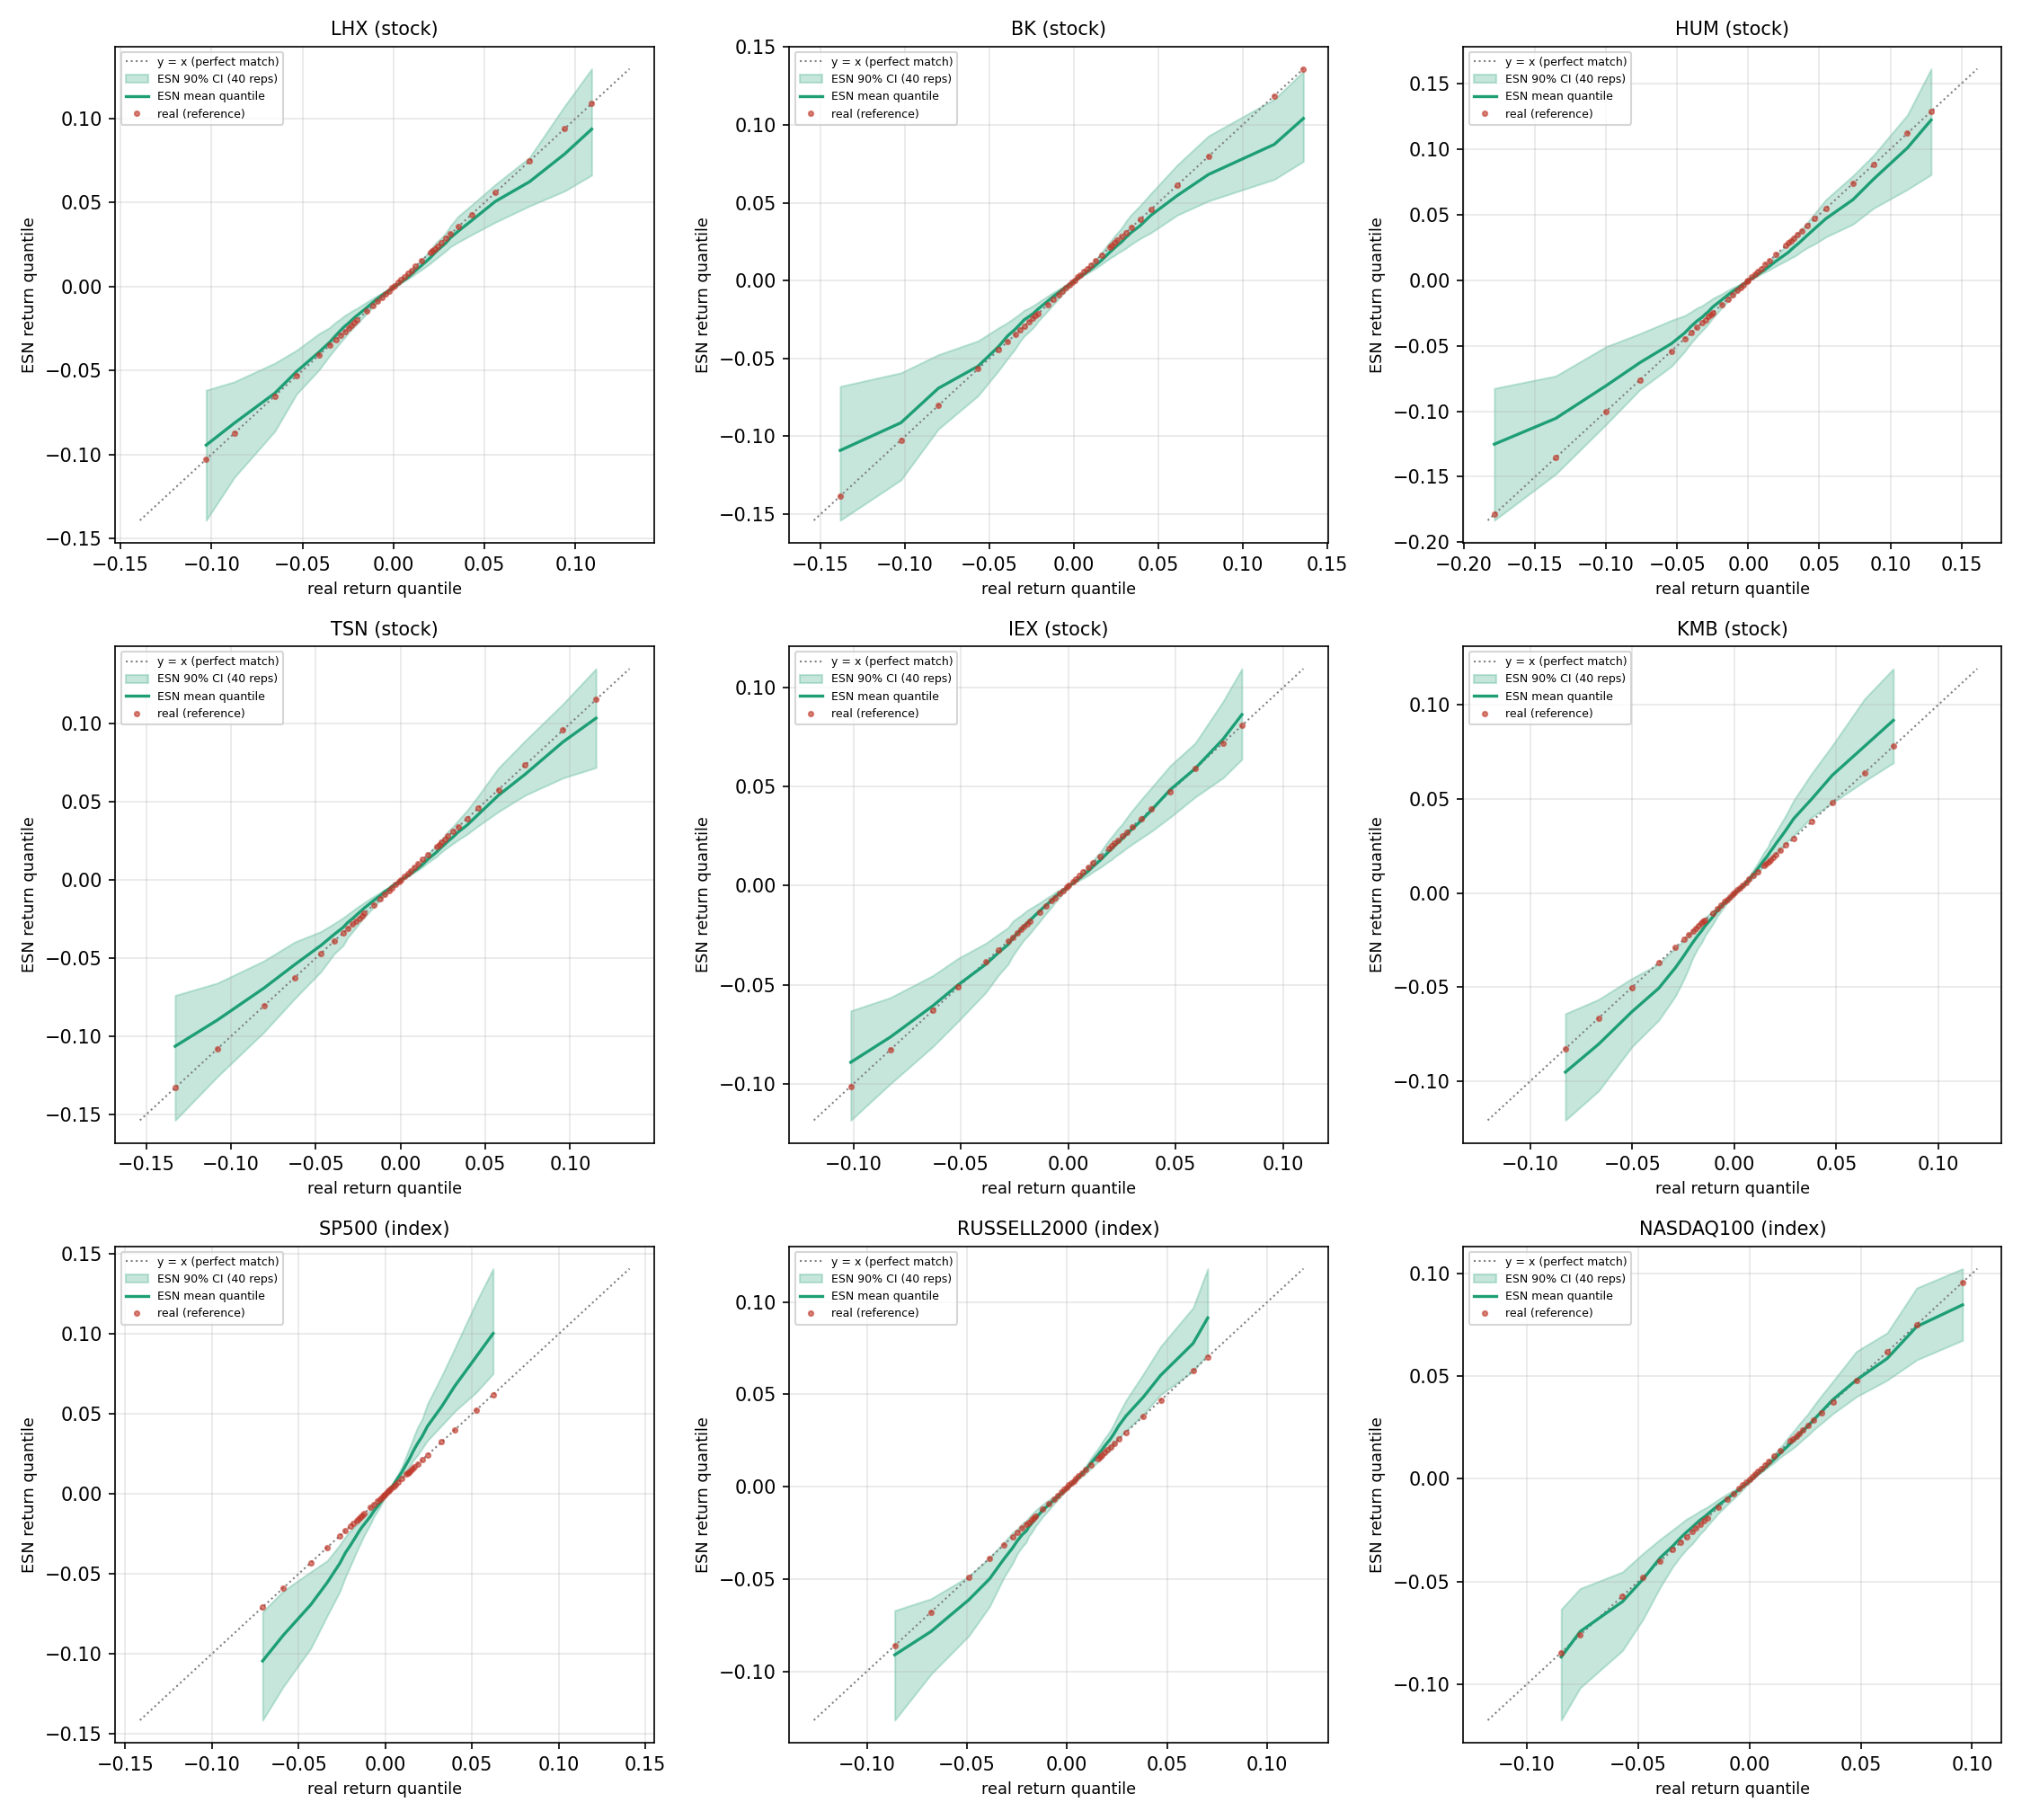
\includegraphics[width=0.98\textwidth]{kurtosis_qq_bench9.png}
\caption{Quantile-quantile plot: real return quantile (horizontal axis) vs.\
the calibrated ESN's own quantile at the same probability level (vertical
axis) -- mean (green) and $90\%$ confidence band (shaded, 40 replicate
$T=4{,}000$-day paths) -- against the $y=x$ reference line (dotted) a
perfect distributional match would follow, all 9 assets.}
\label{fig:kurtqq}
\end{figure}

\textbf{For most assets, the calibrated ESN's own mean quantile curve tracks
$y=x$ closely through the centre of the distribution and for moderate
quantiles}, consistent with \S\ref{sec:fixmethod}'s finding that overall
kurtosis is well matched. \textbf{At the most extreme quantiles, several
assets show a visible, asymmetric deviation from $y=x$} -- most clearly
\texttt{SP500} and \texttt{HUM}, where the calibrated ESN's own left-tail
quantiles sit noticeably below the $y=x$ line (a fatter left tail than real
data shows at that same probability level) while the right tail tracks more
closely. \textbf{This is a genuinely different check than kurtosis alone
can make}: a single scalar summary cannot see whether a good overall match
is actually 2 tails matching individually, or one tail overshooting while
the other undershoots by a similar amount -- the same caution the
Taylor-effect and Zumbach-effect notes' own component-level checks raised
for their own single-scalar and difference-based objectives.

\FloatBarrier
\subsection{The full return distribution, directly}
\label{sec:distribution}
Figure~\ref{fig:kurtdist} shows the same comparison a third way: the full
empirical density of standardised returns (each series shifted to zero mean
and scaled to unit standard deviation), real asset against a large pooled
sample from the calibrated ESN (40 replicate paths, $T=4{,}000$ days each,
$160{,}000$ points in total per asset -- far more than any single real
series, so the ESN's own histogram is a much smoother, more stable estimate
than the real one, which is comparatively noisy this far into its own
tails). Plotted on a log density scale so that agreement or disagreement in
the tails, not just the bulk, is visible directly.

\begin{figure}[h]
\centering
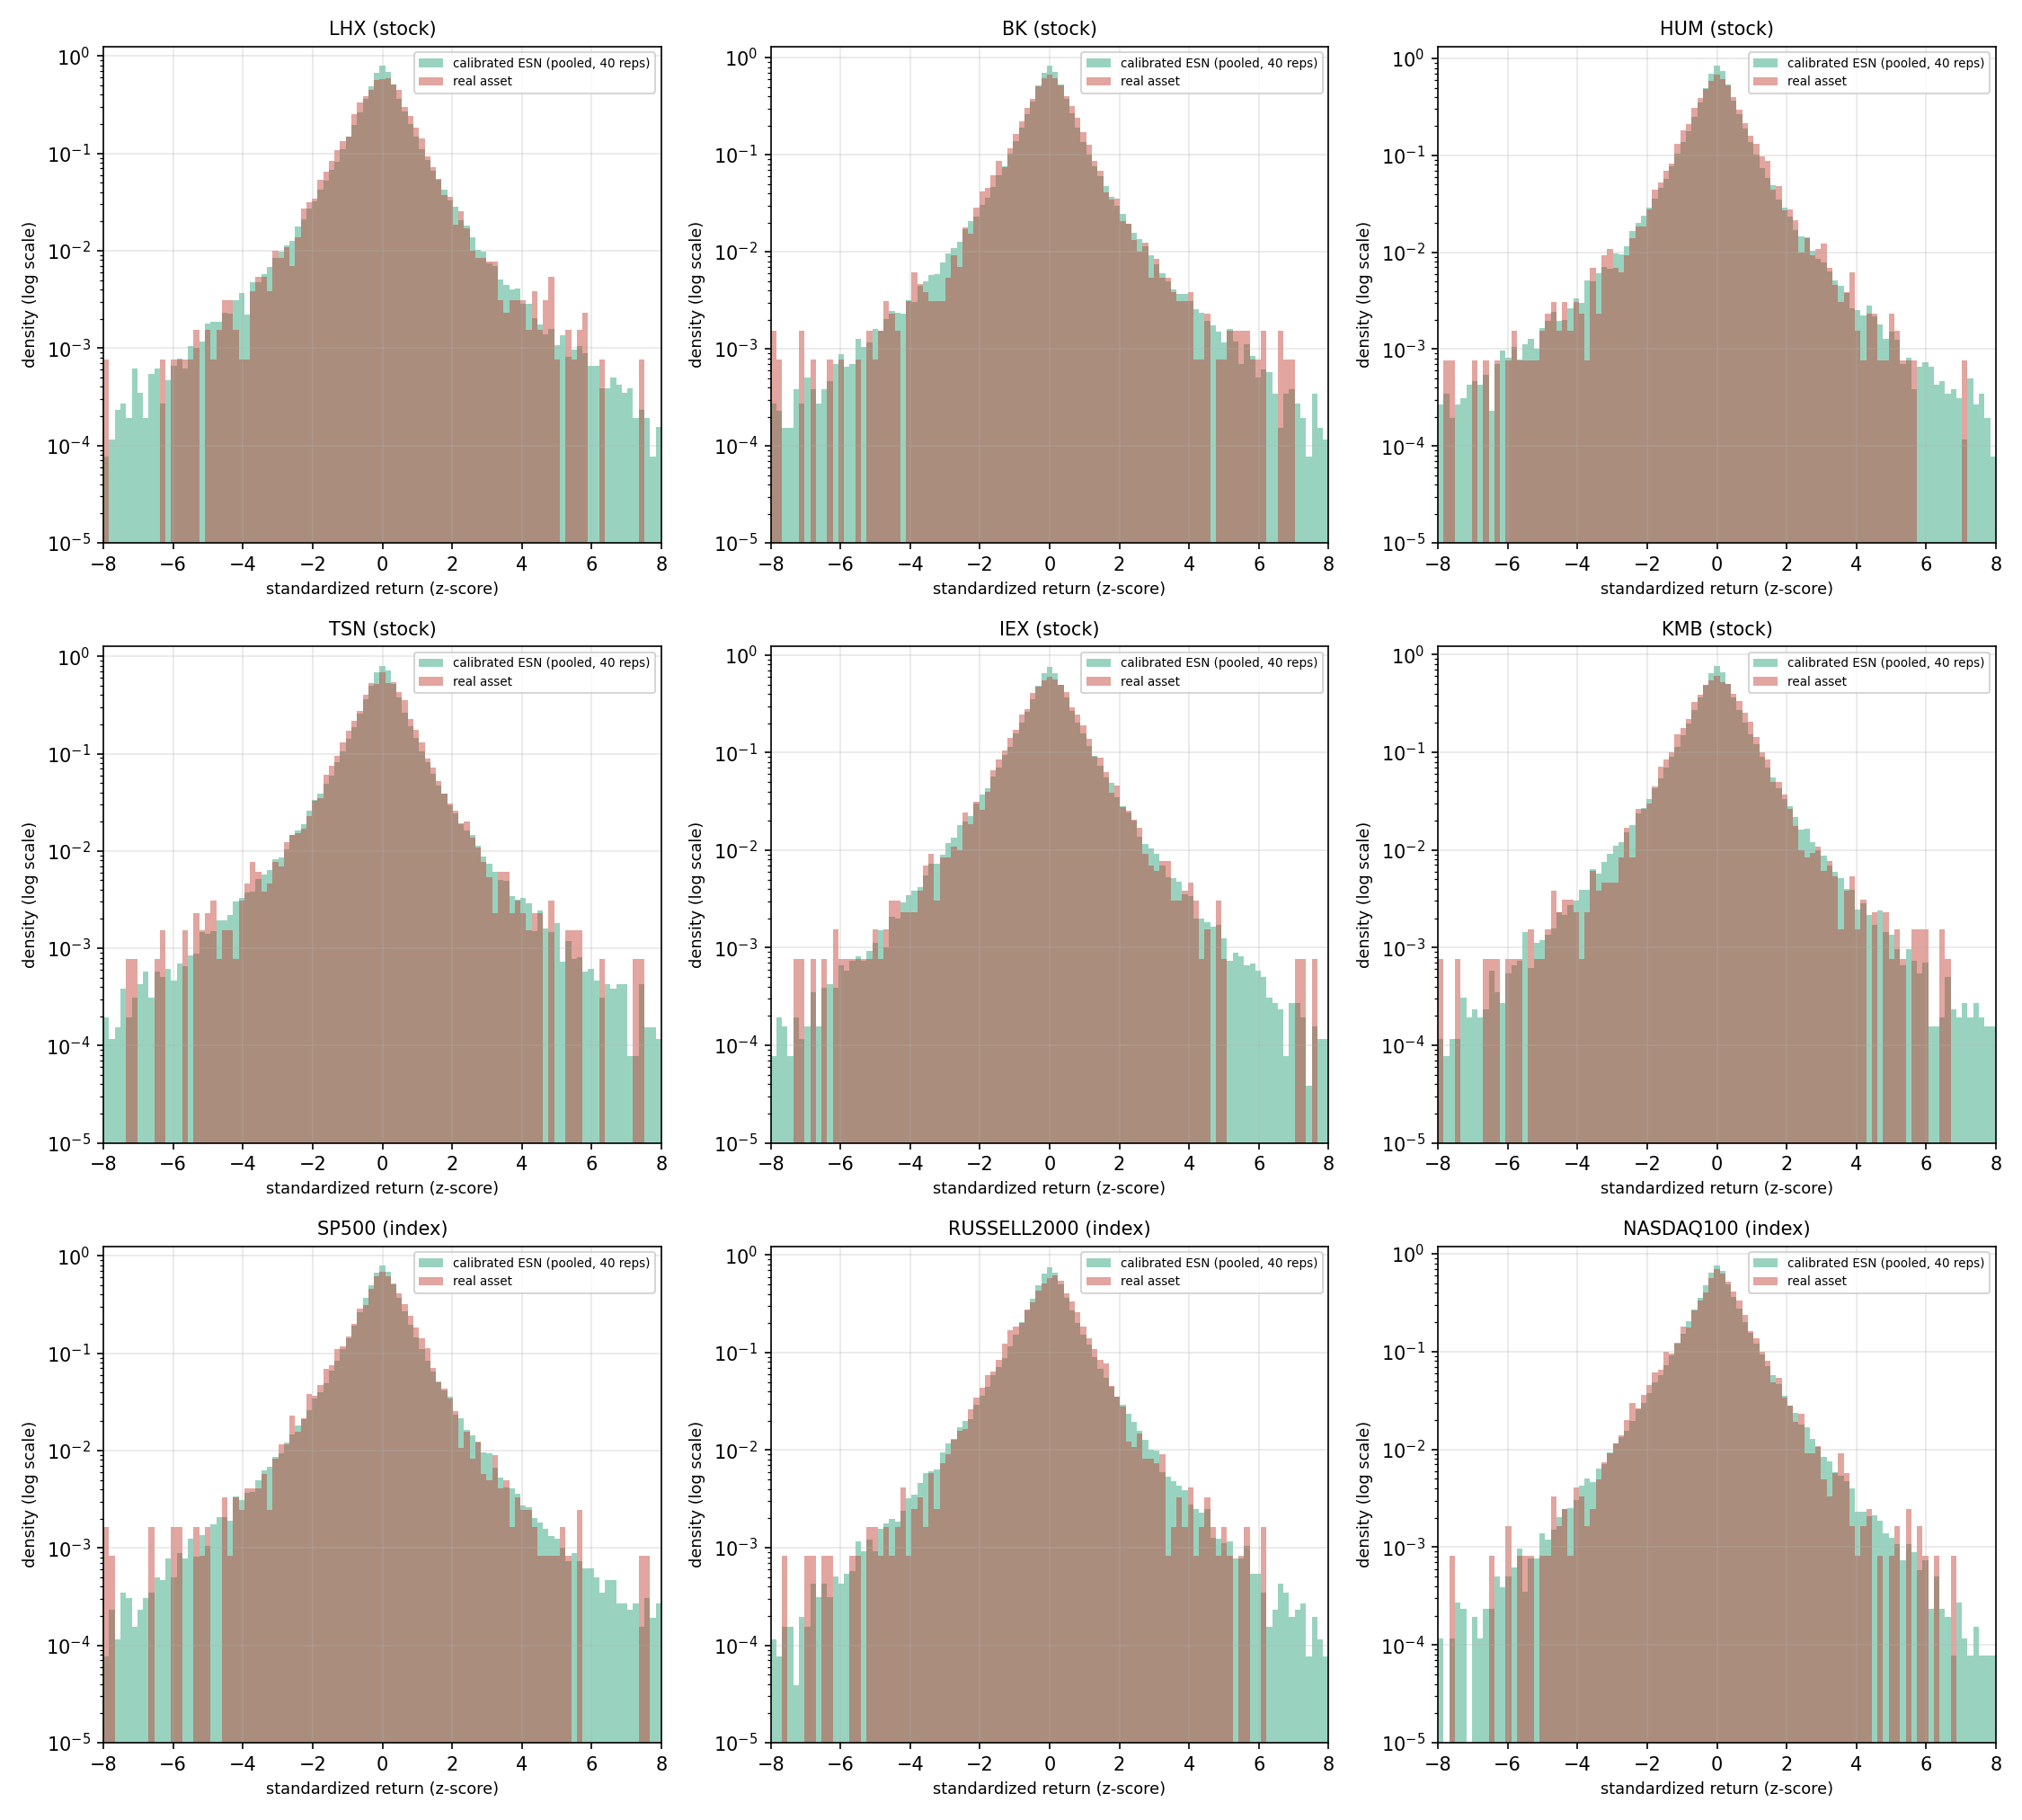
\includegraphics[width=0.98\textwidth]{kurtosis_distribution_bench9.png}
\caption{Standardised return distribution (log density scale): real asset
(red) vs.\ the calibrated ESN's own pooled sample (green, 40 replicate
$T=4{,}000$-day paths), all 9 assets.}
\label{fig:kurtdist}
\end{figure}

\textbf{The 2 distributions overlap closely across their full range for
every asset}, including several orders of magnitude down into the tails --
a direct visual confirmation of \S\ref{sec:qq}'s own quantile-level finding
that the centre and moderate quantiles match well. The asymmetric tail
mismatch \S\ref{sec:qq} identifies for \texttt{SP500} and \texttt{HUM} is
visible here too on close inspection (the green histogram's own left tail
extends slightly beyond the red one at the same density level for those 2
assets specifically), but is subtle at this view's own resolution compared
to the QQ plot's more sensitive, quantile-by-quantile comparison.

\FloatBarrier
\section{Interpretation}
\textbf{The heavy-tailedness gap, like the front-loading, persistence
ceiling, and remaining offsets found in this note family's other 3 notes,
turned out to be reachable within the existing 4-parameter family plus one
already-defined but never-freed parameter} -- not a fundamentally missing
mechanism. Unlike those 3 notes, though, the relevant lever here is
$m_1$, not $H$ or $\lambda_{hi}$: the same "good corner" that fixed leverage,
the Taylor effect, and the Zumbach effect already supplies more kurtosis
than most real assets need, and $m_1$ provides clean, bidirectional control
around that baseline. \textbf{The optimisation itself needed a different
approach here, too}: kurtosis's own high estimation variance defeated a
direct 5-dimensional gradient search that had worked for every other
stylised fact in this note family, and fixing 4 parameters to solve a
well-behaved 1-dimensional problem for the 5th was the more reliable path,
not a lesser one.

\section{Limitations and Recommended Next Steps}
\begin{enumerate}
\item \textbf{$H,\texttt{rough\_scale},\lambda_{lo},\lambda_{hi}$ were fixed
at a single shared corner for every asset, rather than calibrated
individually.} Whether allowing these 4 to vary per asset alongside $m_1$
would improve the fit further, once the underlying 5-dimensional
optimisation difficulty (\S\ref{sec:firstattempt}) is addressed some other
way (e.g.\ many more paths per evaluation, or a derivative-free method
better suited to a noisy objective), was not tested.
\item \textbf{\texttt{IEX} and \texttt{NASDAQ100} calibrate to $m_1$'s own
lower bound}, $-0.1$, without exactly reaching their own (lowest) real
targets. Whether a wider lower bound would let $m_1$ push further and close
this fully, following the same "the bound, not the model, was limiting"
pattern found for $H$ and $\lambda_{hi}$ in this note family's other
documents, was not tested here.
\item \textbf{$m_2$, the other quadratic coupling term in $\eta_t$, held at
its own midpoint of $0$ throughout, was not tested as an alternative or
additional lever.} A brief sweep (in this note's own supporting code) found
$m_2$'s own effect on kurtosis much weaker than $m_1$'s, but a joint
$m_1,m_2$ calibration was not attempted.
\item \textbf{The confidence bands are wide} (Figure~\ref{fig:kurtcalibrated}
shows some spanning close to an order of magnitude), reflecting kurtosis's
own genuinely high estimation variance rather than a calibration weakness --
but this also means the calibration's own precision cannot be judged as
tightly as for the other stylised facts in this note family.
\item \textbf{The asymmetric tail mismatch \S\ref{sec:qq}'s QQ plot reveals
for \texttt{SP500} and \texttt{HUM} specifically was not resolved.} $m_1$
moves both tails together (it enters $\eta_t$ through $\lVert r_t\rVert^2$,
an even function with no left/right asymmetry of its own); a genuinely
different lever -- e.g.\ allowing \texttt{rough\_orientation}'s own sign to
vary, or freeing $m_2$ alongside $m_1$ -- would likely be needed to separate
the 2 tails, and was not tested here.
\item \textbf{The 6 stocks and 3 indices were not chosen for any particular
economic or sectoral reason} -- the stocks are an independently randomised
selection (seed 2026), and the indices are the only 3 with available OHLC
data.
\end{enumerate}

\end{document}
